%!TEX root = ../thesis.tex

\graphicspath{{Chapter2/Figures/}{Chapter2/Tables/}{Chapter2/Charts/}}
\setlength{\parskip}{2ex}

\chapter{Related Work}

\section{Introduction} %Section - 2.1 
As outlined in the introduction, this thesis focuses on how software team size and stability impact the internal structural attributes of software. Out of this come three individual strands of related work which will be the focus of this chapter. 

The first part of this chapter reviews the studies of the impact of people factors on the externally observable attributes of software, with a focus on factors of team size and stability. This work has the greatest direct relevance to this research and is one that this thesis endeavours to further by offering an alternative approach based on the direct measurement of the internal structural attributes of software rather than the observation of external attributes. The second strand of related work in this chapter comprises the body of research that establishes correlations between the internal structural metrics of software and its external attributes. This is of crucial relevance to this work as it is that very body of research that will later be relied upon to map observable trends of structural metrics onto conclusions that have meaning from the perspective of a non-technical stakeholder with a sole interest in the external attributes of the software. The third strand of related work concerns the practicalities of mining software repositories. A survey is provided of the available tools and a summary of the pertinent challenges and pitfalls associated with mining software repositories.

\begin{figure}[htbp!] 
\centering    
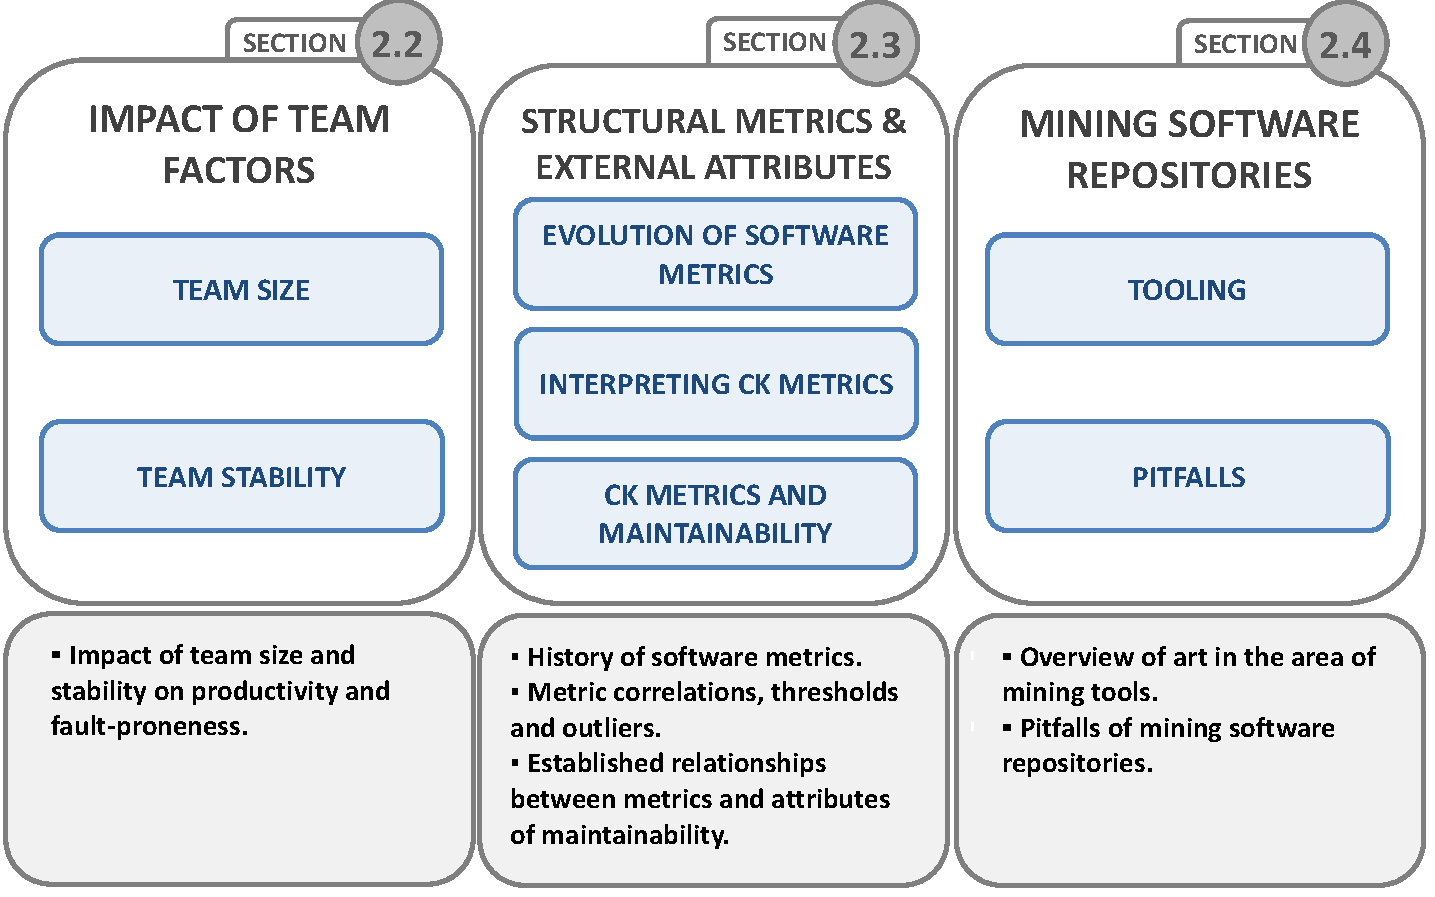
\includegraphics[width=1.0\textwidth]{ChapterOverview.pdf}
\caption{Chapter 2 outline providing an overview of the contents of each section.}
\label{fig:ChapterOverview}
\end{figure}

\section{The Impact of Team Factors} %Section - 2.2
There is a significant corpus of existing work concerned with establishing the impact of factors of team composition on the external attributes of software. This body of research models the relationship between developer and organisational factors with aspects such as fault-proneness and team productivity. This work provides the basis for the null hypotheses detailed in the previous chapter as well as the empirical approach of this study as we adopt and adapt previously established measures of team size and stability. 

\subsection{Team Size}
There have been several empirical studies investigating the relationship between development team size and the team productivity. In his popular book 'The Mythical Man Month', Brooks argues that, since software development is a complex task, the communication effort is great and adding more developers can lengthen rather than shorten the time taken to complete a task as it adds an exponentially greater number of necessary communication paths between developers \citep{brooks1986mythical} - although it is notable that Hsia et al. \citep{hsia1999brooks} argue that it won't necessarily take longer but will always increase the overall cost of delivery compared with correctly sizing the team from the outset. Roger et al., using data from 130 projects, empirically tested the impact of a number of factors on software development productivity concluding that larger team sizes significantly negatively impact software development time and productivity \citep{rodger2011knowledge}. This is corroborated in other research and using a number of empirical methods \citep{mcleod2011factors, lalsing2012people}. Scholtes et al., using a data set of FLOSS projects, perform network analysis concluding that the magnitude of the productivity decrease is related to the growth dynamics of developer coordination networks \citep{scholtes2016aristotle}. In contrast, Maillart and Sornette find that occasionally an OSS development team will exhibit 'superlinear productivity' in direct relation to the development team size, arguing that occasionally the whole is more than the sum of its parts \citep{maillart2016aristotle}.

Schweik et al. \citep{schweik2008brooks} highlight the need to inform development managers who have a stake in FLOSS projects on whether increasing the development team size is more likely to result in a successful project and help avoid 'project abandonment', arguing that this is the primary tool at their disposal to influence outcomes. Rodriguez et al., acknowledging this impact on outcomes, seeks to advise managers on the ideal team size to facilitate a process of project decomposition and distribution of work amongst appropriately sized development teams \citep{rodriguez2012empirical}. The productivity of teams sized above and below an arbitrary threshold are compared, controlling for the functional complexity of the produced software. In-line with prior literature, it is noted that those teams sized below the threshold are more productive than the larger teams. 

Pendharkar and Rodger investigated the relationship between team size and the associated cost of development \citep{pendharkar2009relationship}. They observed that the team size does not linearly increase software development cost and that, in some cases (hypothesised to be those projects suffering communication inefficiencies), larger teams require a greater than proportional increase in resources. Blackburn et al. make similar observations while also noting that greater functional complexity leads to larger teams \citep{blackburn2006brooks}. This is intuitive given that larger teams have greater knowledge and expertise and therefore would typically be deployed to more complex problems. Hericko et al. worked to define the optimal team size given these two conflicting drivers, proposing a model to minimise development effort for a given project size \citep{herivcko2008approach}.

There has also been research negatively correlating team sizes to measures used as a proxy for software quality. Nagappan used data from Microsoft's Windows Vista project to establish that metrics based on organisational structures (of which team sizes were one aspect) are a significant predictor of software fault-proneness \citep{nagappan2008influence}. Nagappan's work was later validated by Caglayan et al. who found that, while organisational metrics were out-performed by pre-release metrics such as defect counts as a predictor of ultimate fault-proneness, they were a significant predictor nonetheless \citep{caglayan2015merits}. Mockus also noted a correlation between team sizes and fault-proneness \citep{mockus2010organizational}. Bird et al. developed a more sophisticated code ownership model that distinguished between frequent 'major' committers and infrequent 'minor' committers and found that minor committers are more likely to introduce defects \citep{bird2011don}. Bell et al. observed that the number of developers that modify a file increased the probability of that file being defect prone \citep{bell2013limited}. Recently, Chopra et al. and others have moved this research forward by building prediction models to identify fault-prone classes built upon a number of predictors including team size \citep{madeyski2015process, chopra2018empirical}.

\subsection{Team stability}
Team stability (in literature also referred to as  'team familiarity' or by the antonym 'team fluidity') is also viewed as a critical success factor for an effectively functioning and performing group wherever complex problems are tackled. From cardiac surgery teams to flight crews and basketball teams, those teams that experience continuity in personnel make-up are likely to be higher performing \citep{carthey2001human, akgun2002antecedents, yeh2005influences, wiegmann2010improving, huckman2013hidden, joshi2018should}. Software development teams are no exception \citep{bao2017will}. The Scrum Agile software development methodology, for example, favours avoiding changing team members for the stated reason that stable development teams are more productive \citep{deemer2010scrum}. There is anecdotal evidence to back this claim up with practitioners reporting that fluid teams are likely to be less productive as they tend to go through the 'Tuckman cycle' (Forming, Storming, Norming, Performing) with the addition of every new team member \citep{tuckman1965developmental, linders2011establishing}.

There has been comparatively few academic studies investigating the role of team stability within the field of software development. On the empirical side, Huckman et al. conducted a detailed study of the team stability and role experience on the output of development teams \citep{huckman2009team}. Armed with a data set of over a thousand projects and defining team success criteria in terms of software defect count and adherence to deadlines and budgets,  they found that a conventional measure of experience - years of experience at a firm - was not linked with team performance. However, team stability (measured as the average number of times that each member has worked with every other member of the team) was associated with less error-proneness and more budget adherence. One stark result was that, as familiarity increased by 50\%, defects decreased by 19\%, and deviations from budget decreased by 30\%. This was confirmed by Gardner et al. who observed that teams with a high degree of team stability, captured by measuring the length of time that each team member had worked with their teammates, yielded a 10\% increase in client satisfaction \citep{gardner2012dynamically}. Mockus, studying a large commercial software project, observed that new developers were not associated with a decrease in quality (postulating that this was due to new developers being assigned peripheral tasks) while departures from the project were associated with greater fault-proneness \citep{mockus2010organizational}.
 
\section{Structural Metrics and External Attributes} %Section - 2.3
Underpinning the empirical approach to this research is the use of structural metrics to measure the internal attributes of software. This section discusses the evolution of software metrics, efforts to interpret metrics, and research modelling the impact of structural metrics on maintainability. The latter is particularly relevant as these relationships will be drawn upon later in this thesis to infer the likely impact of observations of structural metrics on the external attributes of the studied software systems.

\subsection{Evolution of Software Metrics}
The study and application of software metrics dates back to the mid-1960's when the primitive Lines of Code metric was routinely used as the basis for measuring software development productivity (developer LoC per month) and quality (defects per KLoC). In 1971 Akiyama proposed the use of metrics for software quality prediction proposing a regression-based model for module defect density (number of defects per line of code) where line of code was used as a crude indicator of complexity \citep{akiyama1971example}. This was one of the earliest attempts, albeit a simplistic one, to extract an objective measure of software quality through the analysis of artefacts of a system. With the increasing diversity of programming languages, it became necessary to introduce a more sophisticated model of the structural attributes of software. 

McCabe, recognizing the importance of testable and maintainable software systems, broke new ground in the area of software metrics introducing the first meaningful structural metrics \citep{mccabe1976complexity}. In 1976, motivated by the observation that half the development time is spent in testing and that most of the cost of owning a system is in its maintenance, he developed a software metric which he termed 'cyclomatic complexity'. This metric is based on a formula to calculate the number of linearly independent paths through source code. Its purpose is to identify complex software modules based on program flow. Around the same period Halstead designed a structural metrics suite based on definitions of operators and operands modelling the complexity of individual lines of code \citep{halstead1977elements}. To give a flavour of these metrics, the Halstead Difficulty uses a formula to assess the complexity based on the numbers of unique operators and operands capturing a measure of how difficult the code is to write and maintain. Halstead Effort is an estimate on the effort to rewrite a particular method.

The research community continued to be highly active in the field of structural metrics throughout the next decade \citep{cote1988software} with advances in the usage of existing 'classical' metrics \citep{behrens1983measuring, gaffney1981metrics} as well as the formulation of new structural metrics \citep{boydston1984programming, prather1984axiomatic}.

In the 90s, with the increasing adoption of Object-Oriented (OO) programming languages, the research in structural metrics took another significant step forward. Chidamber and Kemerer argued that Object-Orientation, as the most prominent advance in software development, and with yet to be established practices, necessitated measures that could guide organizations to its successful adoption. This fact, coupled with criticisms of existing metrics suites, saw the development of the Chidamber and Kemerer (CK) metrics suite, detailed in Table ~\ref{tab:ckmetricsuite} \citep{chidamber1991towards, chidamber1994metrics}. For its popularity and simplicity, as detailed later in this chapter, this is the suite that will be used to underpin the empirical work in this thesis.

\begin{table}
\captionof{table}{A summary of the CK metric suite.}
\begin{tabular}
 \centering 
 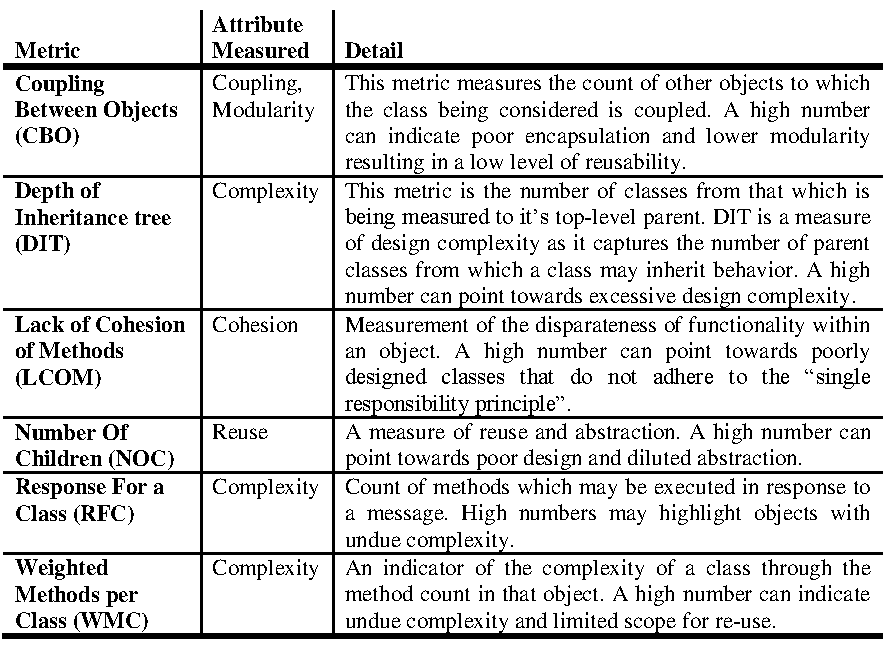
\includegraphics{CKMetricSuite.pdf}
 \label{tab:ckmetricsuite}
\end{tabular}
\end{table}

\subsection{Interpreting CK metric values}
At a time when OO metrics were a relatively new field of study, Rosenberg proposed that metrics without interpretation guidelines are of little value. She concluded that, although some numeric thresholds were suggested by developers, there was little to justify specific values \citep{rosenberg1998applying}. She proceeded to harness experiences within the NASA Software Assurance Technology Centre (SATC) to apply a common sense approach to the formulation of interpretation guidelines of individual OO metrics including most of the CK suite. These findings are summarized in Table ~\ref{tab:rosenberg}. The table shows the objective  - the direction of trends associated with favourable outcomes - and the associated impact on the external attributes. For instance, it was concluded that developers should attempt to attain low values of LCOM (the objective), which will result in a higher degree of understandability, maintainability and reuse, while reducing development effort. 

\begin{table}
\captionof{table}{A summary of the Rosenberg OO metrics guidelines.}
\begin{tabular}
 \centering 
 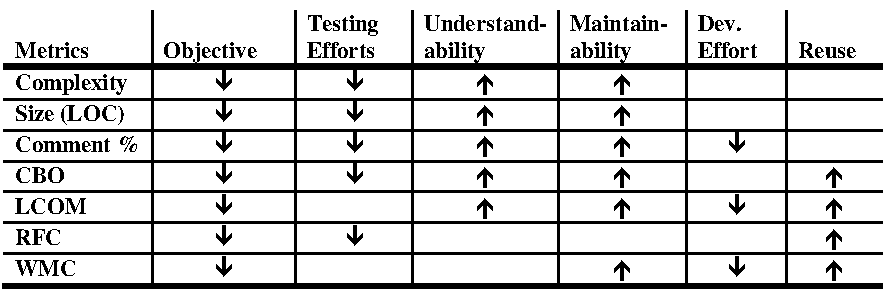
\includegraphics{Rosenberg.pdf}
 \label{tab:rosenberg}
\end{tabular}
\end{table}


However pertinent and useful, Rosenberg's research was based on the knowledge and experience within SATC, and was not an empirical treatment of software metrics. Shatnawi moved this area of metrics research forward by establishing CK metric threshold values at a number of risk levels representing probabilities of error proneness \citep{shatnawi2010quantitative}. Oliveira et al. worked to devise a technique to establish relative thresholds across a corpus of 79 projects programmed in Pharo and Smalltalk, identifying those projects that violated thresholds for a higher percentage of metric observations in order to find projects which would be expected to exhibit lower maintainability \citep{oliveira2015validating}. Hussain et al. used logistic regression to identify thresholds above which classes exhibit greater fault-proneness \citep{hussain2016detection}.

Chidamber et al. researched the question of the interpretation of the CK metric suite for managerial use and concluded that 'outlier' metric values indicate a level of complexity that would require management action \citep{chidamber1998managerial}. Chidamber et al. continued to suggest that a useful method to identify such 'outlier classes' is by applying Pareto's 80/20 principle and selecting classes which exhibit metric values from the 80th percentile for further attention - for example assigning a higher skilled developer to that implementation or assigning extra testing resources to that component.

Basili et al, motivated by the objective to leverage structural metrics to provide guidance to the areas of a system where testing efforts are best spent, established the utility of the Chidamber and Kemerer suite as a predicator of fault-prone software classes  \citep{basili1996validation}. This was achieved by assembling eight software development teams and using regression analysis to establish relationships between OO metrics and observed defects. 

These are, by no means, the only studies of this nature. Subramanyam and Krishnan conducted similar work with access to a large number of in-house developed codebases, controlling for programming language and software size, confirming the results obtained by Basili et al \citep{subramanyam2003empirical}. These results were further validated in a number of similar studies, each adding its own unique contribution \citep{el1999validation, tang1999empirical, cartwright2000empirical, el2001prediction, subramanyam2003empirical, gyimothy2005empirical, xu2008empirical, malhotra2012fault, okutan2014software, song2018comprehensive}. Table ~\ref{tab:FaultModels} surveys the empirical approach within this research.

\begin{table}
\captionof{table}{A survey of the research modelling fault-proneness as the dependent variable and CK metrics as the independent variables.}
\begin{tabular}
 \centering 
 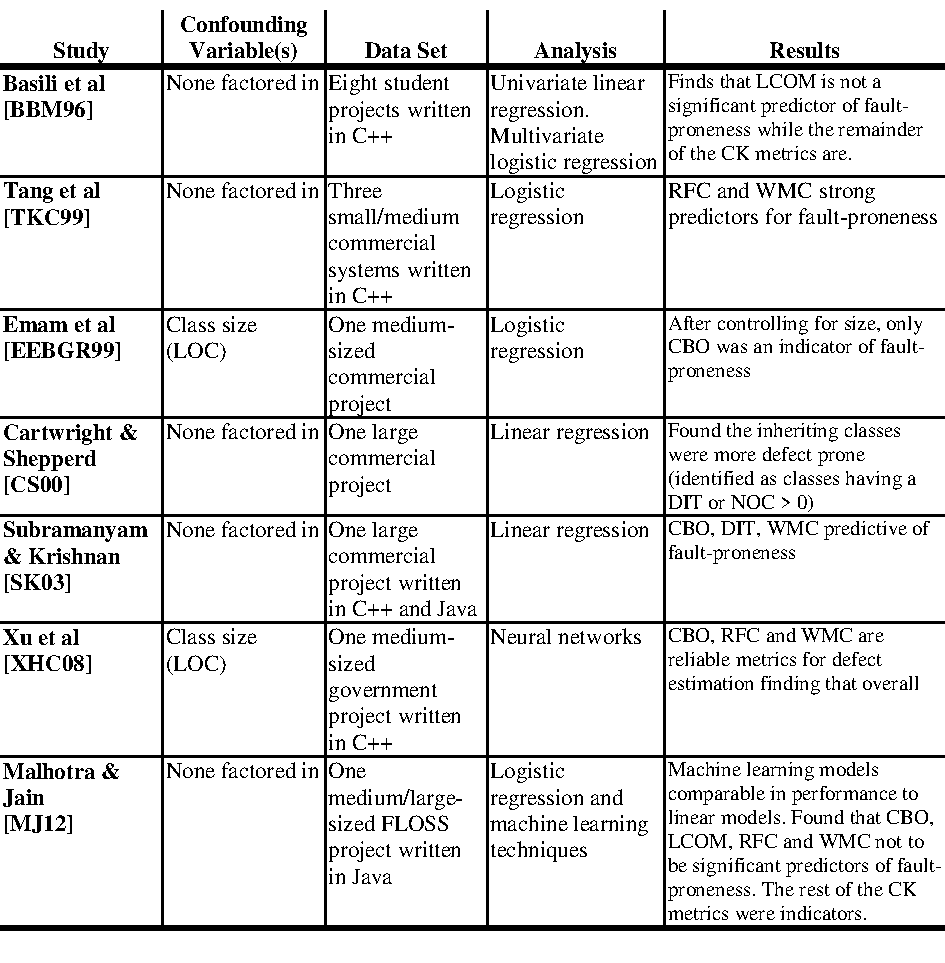
\includegraphics[width=1.0\textwidth]{FaultModels.pdf}
 \label{tab:FaultModels}
\end{tabular}
\end{table}

Saberwal et al. developed logistic regression models relating CK metrics to bad code smells driven by the desire to guide refactoring efforts to where they are most needed \citep{saberwal2013empirical}. More recently, this work was validated by Tufano et al. \citep{tufano2017and} using linear regression models. Badri et al, using similar techniques, concluded that a correlation exists between LCOM and unit test coverage, validating the use of OO metrics as a predictor of the testability of classes \citep{badri2011empirical}.

\subsection{CK metrics and Maintainability}
Santos et al and Ernst independently identified a number of issues with threshold values, foremost among them that these values make generalised statements across projects \citep{Santos2017AnES, ernst2018bayesian}. Structural metric values depend heavily on complexity and size, and therefore a single threshold value will not necessarily hold true across a diverse set of projects. Moreover, establishing a threshold across a corpus of projects using the techniques devised by Oliveira et al. is arguably of limited value to this research given the objective of establishing inferences from metric trends on how software maintainability is generally impacted by team factors. For this reason, this section focuses on surveying the research that empirically establishes a relationship between CK metric values and externally observable attributes of software in order to expand upon (and detail the empirical validation of) Rosenberg's interpretation of the relationship between CK metrics and maintainability.

As established in the previous chapter, maintainability is comprised of four sub-attributes - analysability, changeability, stability, and testability. Correia et al, through a survey-based study present the opinion of software quality experts that a number of structural attributes drive the sub-attributes of maintainability \citep{correia2009survey}, the consensus being that size, complexity, coupling, cohesion and test quality are all key factors. Chong and Lee developed a technique to visualise the structural attributes of codebases using a weighted complex network in order to capture its structural characteristics, with respect to its maintainability and reliability \citep{chong2015analyzing}. They broadly observe that high coupling and low cohesion are associated with lower maintainability, confirming the consensus of the software quality experts. Li and Henry conducted one of the first studies to determine if CK metrics could be used as a predictor of maintenance effort, concluding that DIT, LCOM, NOC, RFC and WMC all predict maintenance efforts beyond what can be predicted for size alone \citep{li1993object}.

The next section surveys research modelling the relationship between CK metrics on particular sub-attributes of maintainability and each of the sub-attributes of maintainability.

\subsection{CK metrics and the Sub-Attributes of Maintainability}
Bruntink and van Deursen used correlation analysis to study the relationship between CK metrics and the testability of software using a data set of five projects (including one open-source project) \citep{bruntink2006empirical}. Using the lines of test code and the number of test cases in the unit tests as a proxy for testability, they find that DIT, LCOM and NOC are predictors of testability. It is attributed by the authors to be due to the developers choosing not to re-test inherited behaviour from the parent class within each child class. Badri et al. furthered this research by testing a series of metrics capturing the structural attribute of cohesion for correlation (of which LCOM was one) against testability \citep{badri2011empirical}. Confirming the results of Bruntink and van Deursen, LCOM was found to be a significant predictor of testability. 

Harrison et al. used a similar statistical approach to confirm a negative correlation between WMC and the time to create automated tests for software \citep{harrison1998investigation}. 

Harrison et al. also broadened the scope of their research to cover understandability and changeability. To measure software understandability, a model formulated by Boehm et al. is used which rates software qualitatively on its structure, application clarity and self-descriptiveness \citep{boehm1978characteristics}. A simplified version of this model is replicated in Table ~\ref{tab:bohem}. Harrison et al. measure the time to implement modifications as a proxy to measuring changeability. WMC was found to be negatively correlated with understandability. Both WMC and LCOM were negatively correlated with changeability.

\begin{table}
\captionof{table}{A reproduction of Boehm's software understandability model.}
\begin{tabular}
 \centering 
 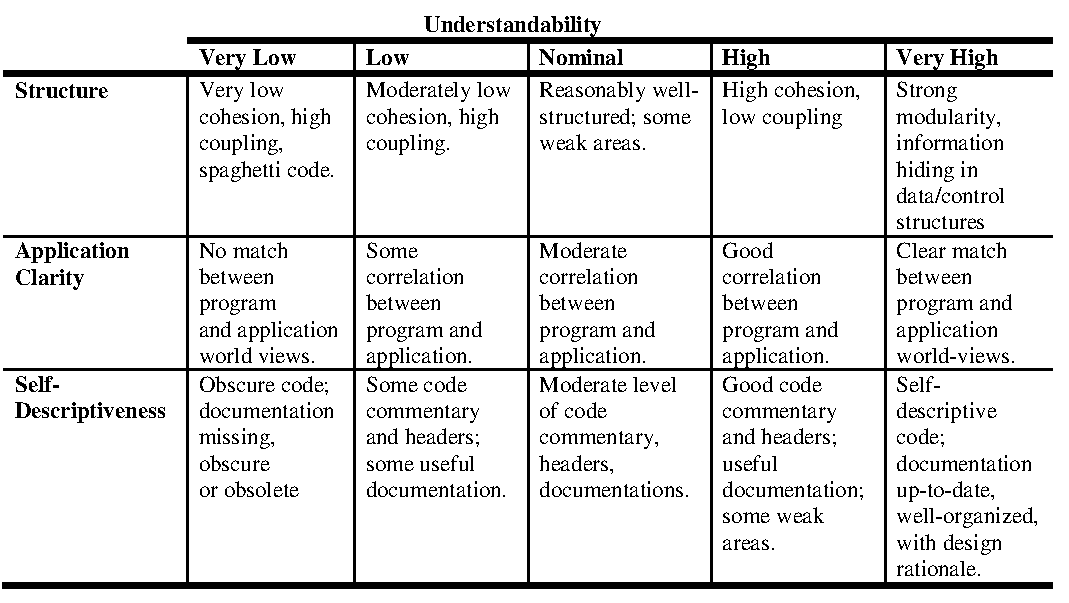
\includegraphics[width=1.0\textwidth]{BoehmUnderstandabilityModel.pdf}
 \label{tab:bohem}
\end{tabular}
\end{table}

Elish and Rine conducted a study to determine if CK metrics could be used as a predictor of the stability of software \citep{elish2003investigation}. Their research calculated the class-level stability through an algorithm that determined the likelihood that the class would be change-prone as a result of a class-level change elsewhere in the design. 

CBO, DIT, LCOM, RFC, and WMC were all found to be negatively correlated with stability. In particular CBO and RFC were strong predictors of stability. A high CBO indicates that a class depends on many other classes or that many other classes depend on it, increasing the likelihood that change ripples through to the high CBO class. Similarly, a class with a high RFC indicates a higher number of internal and external methods that may impose change on the class. 

Tables ~\ref{tab:MaintainabilitySubatrributes} and  ~\ref{tab:MaintainabilityModels} provide a summary of this survey. This will be drawn upon later in this thesis to draw insights from observations on structural metrics trends in the context of their impact on maintainability.

\begin{table}
\captionof{table}{A summary of established associations between CK metrics with the sub-attributes of maintainability.}
\begin{tabular}
\centering 
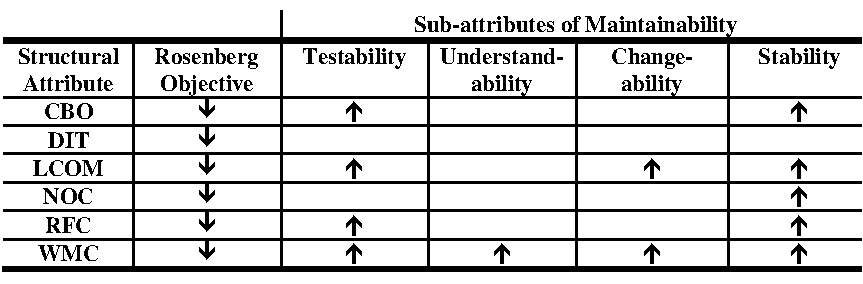
\includegraphics{MaintainabilitySubatrributes.pdf}
\label{tab:MaintainabilitySubatrributes}
\end{tabular}
\end{table}

\begin{table}
\captionof{table}{A survey of the research establishing  associations between CK metrics with the sub-attributes of maintainability. No confounding factors are controlled for.}
\begin{tabular}
\centering 
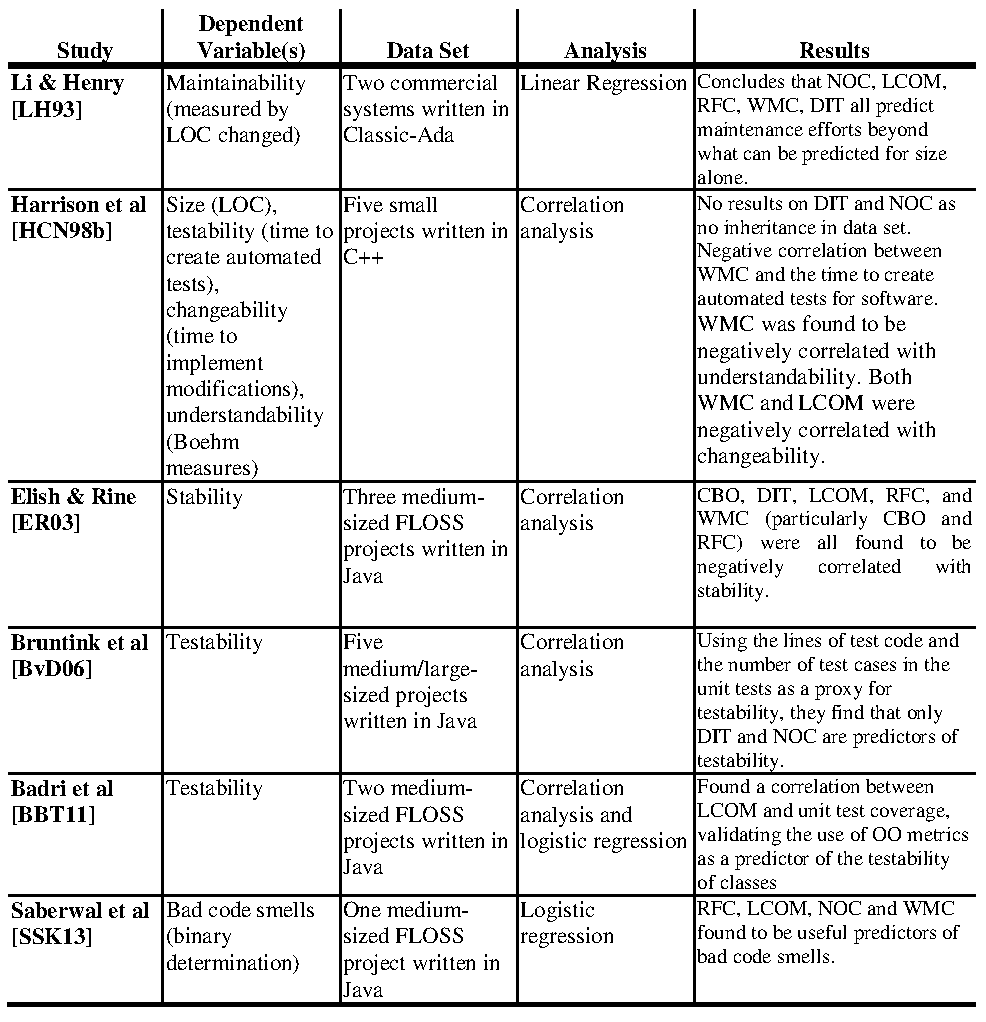
\includegraphics[width=1.0\textwidth]{MaintainabilityModels.pdf}
\label{tab:MaintainabilityModels}
\end{tabular}
\end{table}

\section{Mining Software Repositories} %Section - 2.4
The field of mining software repositories is a broad and active research area. Researchers typically inspect particular characteristics of a system throughout its evolution and observe trends and relationships. Kagdi et al. classify these types of studies into one of two categories \citep{kagdi2007survey}. The first category of investigations observes the changes in properties through multiple versions of a system - for example, defect density or software complexity \citep{yamashita2017software, agrawal2018we, tian2018statistical}. The second category of investigation is more interested in the mechanics of the changes in artefacts - for example who is revising source files, how often, and the drivers of change \citep{lee2017understanding, ortu2018mining}. This research is focused on mining software repositories to study changes in properties.

This section reviews the related work in three areas. A survey is provided of the prior research mining and analysing forges - those centralised platforms such as SourceForge, GitHub and GoogleCode which provide the ecosystem to facilitate distributed development. Then a survey of the tools that have been developed to support the activity of mining software repositories is presented and evaluated in the context of its applicability to this research. Finally, the challenges and pitfalls associated with mining individual project repositories or entire forges are then discussed with an emphasis on aspects of network analysis and accurately determining authorship.

\subsection{Forges}
There have been a number of studies where a multitude of repositories have been mined within a broader forge. These studies have typically focussed on analysing project artefacts to study the impact of developers, the forge, or to otherwise facilitate the process of FLOSS adoption.

Eilhard and M{\'e}ni{\`e}re conducted an empirical study of 10,533 projects on SourceForge assessing the productivity of development team members, finding that volunteers tend to score lower than corporate developers \citep{eilhard2009look}. Similarly corporate developers are found to benefit more from 'knowledge spillover' - the positive exchange of information between individuals within an organisation. Capiluppi and Beecher carried out a comparative analysis between two large forges - Debian and SourceForge - to assess whether the decay of software architecture is impacted by the forge \citep{capiluppi2009structural}. While Debian was found to host more complex projects, it also exhibited greater 'anti-regressive' work to reduce this complexity over time. Capiluppi et al. also attempted to identify whether the forge could have an impact on the structural metrics of the developed software \citep{capiluppi2009quality}. They find no significant difference between metrics on the KDE forge (which specifically reinforces coding standards) compared with SourceForge (which does not do so). 

Bagnato et al. state that assessing if a FLOSS project meets the requisite standards for business adoption is a non-trivial task and requires analysis of multiple project artefacts including source code, documentation and issue trackers \citep{bagnato2017developer}. To support this process, they developed an IDE plug-in called CrossMiner which extracts information from these various data sources for a given project and presents it within a single screen. In a similar vein, Wasserman et al. developed a methodology and a tool to assess the 'business suitability' of FLOSS projects by, again, mining these data sources and rating projects on a series of criteria including  functionality, documentation and adoption \citep{wasserman2017osspal}. More recently Tamburri et al., also motivated by the need to provide greater rigour around the process of FLOSS adoption developed a tool called 'Yoshi' to analyse the open-source community and categorise it into one of a number of known organisational patterns \citep{tamburri2018discovering}. Applying their analysis to 25 projects from GitHub, they assert that they find value in measuring and monitoring these key organisational aspects. 

\subsection{Mining Tools}
With the advent of open-source repositories, researchers acquired access to an large and rich data set. This led to an improvement in the tooling used to mine repositories. German \citep{german2004mining} documented the challenges involved in mining the CVS repositories of the GNOME project. German et al. \citep{german2005framework} followed this up with a review of some tools the mine repositories and suggested a comparison framework to support this activity. The available tools were generally found to be disparate and fulfil the relatively narrow requirements of the research groups that developed them. More recently Tiwari et al. proposed an 'app store' model for packaging and distributing software repository mining tools utilising their platform 'Candoia' \citep{tiwari2017candoia}. While this platform has not seen significant adoption, the concept is undoubtedly a step forward. In the next chapter a review is provided of the tools of direct relevance to this work and the potential for employing these tools is evaluated in the context of the data extraction and analysis requirements of this research. 

\subsection{Pitfalls}
As will be discussed during the course of this thesis, when mining a significant amount of repository data, there are a number of pitfalls that, where ignored, can constitute a serious threat to the validity of the research. This is an interesting stream of research in its own right and there are a number of studies that typically focus on either a particular VCS or particular challenges that exist across VCS. This is covered  in the next sub-section titled 'Data Extraction and Entity Reconciliation'. Through the course of this research the pitfalls around conducting network analysis in a forge containing forked projects has been a particularly significant challenge and will emerge as dominant theme later in this thesis. Prior research in this area is documented in the sub-section titled 'Forking and Cloning'.

\newline
\textbf{2.4.3.1 Data Extraction and Entity Reconciliation}
\newline
German did some early work in the field of mining software repositories and raised practical concerns with the volumes of data involved in mining a single significant CVS repository, proposing a graphical tool to help visualise large data sets (eventually becoming the SoftChange tool) \citep{german2004mining}. Bird et al. conducted a similar study against the GIT version control system bringing out some its particular idiosyncrasies, particularly around the pervasive nature of branch development and the implications that this has on how to interpret revision history \citep{bird2009promises}.

Also relevant to this work is the research that focuses on the pitfalls associated with mining data from forges. Iqbal et al., attempting to solve for the challenge of integrating data across multiple FLOSS code forges propose the use of so-called 'semantic web' technologies to represent the meta-data contained therein \citep{iqbal2012integrating}. They argue that linking the various developer aliases across forges can produce a holistic picture of their activity, unlocking in the process some useful analytics. To do so they propose an email similarity algorithm which is not fundamentally dissimilar to that used within this research and described in Section 5.2.1 \citep{iqbal2015large}. Goeminne and Mens also highlight the challenges in reliably establishing committer identities across repositories, conducting a survey of a variety of algorithms available to help mitigate this \citep{goeminne2013comparison}. Their work was built upon by Xiong et al. who employed Natural Language Processing to perform identity reconciliation across GitHub and Stackoverflow, the popular developer community-based knowledge base \citep{xiong2017mining, github, stackoverflow}. In a similar vein, Squire tackled the specific problem of identifying projects that reoccur across forges and presented a method to score similarity between project pairs \citep{squire2009integrating}.

Howison and Crowston documented the promises and perils of mining SourceForge, documenting the practical challenges of data extraction, data analysis and research design \citep{howison2004perils}. More recently Kalliamvakou et al. conducted a similar study against GitHub finding that many projects were inactive or have very few commits and most repositories were for individual development \citep{kalliamvakou2014promises}. Some of their work informs the forge and repository analysis documented in Chapters 3 and 4 in an effort to understand the extent that the trends observed in SourceForge and GitHub apply to the forge that is the subject of this thesis: GoogleCode.

\newline
\textbf{2.4.3.2 Forking and Cloning}
\newline
Forking refers to the process of creating an alternate and independent software development stream from an existing project, often retaining the original VCS revision history of the parent. When mining data from projects within open-source forges it is crucial to reliably establish the unique commit activity on a given project and the fact that the forking process duplicates the revision history across multiple projects introduces an avenue of potential distortion to the raw results. When conducting social network analysis, it is essential that each committer's contribution is accurately and reliably identified without threat of misreporting child project engagement when there was only engagement in the parent project. This is particularly true in the case of this research where a particular form team stability is measured by observing the number of previous projects that committers have partnered in. This will be covered in greater detail in Chapter 5.

Nyman and Mikkonen conducted research to establish the most common motivations for forking within SourceForge \citep{nyman2011fork}. The methodology to identify forked projects was to execute a keyword search within project descriptions to find references to forking. Although this approach suffices when attempting to locate a statistically significant  sample to study, relying on developers to specifically declare a project as 'forked' in the description does not help us identify the full set of forked projects.

Robles et al. \citep{robles2006mining} suggested a fairly manual approach for locating significant software forks that involved searching Wikipedia using the term 'software fork' and manually navigating to the project homepage to extract key information ahead of a study on the motivations and outcomes of forking. This is an adequate approach when attempting to extract a sample of forked projects for further study but cannot be applied to the large-scale mining of software forks within open-source forges. More recently, Jiang et al conducted similar research against the GitHub forge and they were able to directly use project meta-data made available by the forge (a recent innovation) to identify forks \citep{jiang2017and}.

As part of the process of maintaining a forked project, it is often desirable or indeed necessary to import changes from the master project. Ray et al. developed a tool called REPERTOIRE to automate the identification of common commits between known forked projects through comparison of source files but it does not attempt to identify forked projects in a wider open-source forge \citep{ray2012repertoire}. This is the most sophisticated approach to detecting forks that is noted in the prior literature. In this general research field there have also been a number of efforts to automate the identification of 'cloned code' i.e. source code that is duplicated within a single project or across projects within a forge. This field of research has drawn some attention due to the potential negative impact that code cloning has on maintainability \citep{lozano2007evaluating}. Lozano and Wermelinger developed a prototype tool called 'CloneTracker' and applied it to the study of changeability within software containing clones \citep{lozano2008assessing}. Clones within a wider forge could indicate the presence of forking, making it valuable input for a heuristic that identifies such projects. Gharehyazie et al. developed a tool called Clone Huntress which identifies code clones in GitHub with the motivation of simplifying 'code foraging' - the process of discovering code within a broader repository that may be of relevance to the 'forager' \citep{gharehyazie2018cross}.

Schwarz et al. \citep{schwarz2012often} developed a set of lightweight techniques based on hashing algorithms to identify cloned code in a way that, in theory, could  scale up to an entire forge. Lee et al. \citep{lee2010instant} developed similar techniques to support instant cloned code researches (albeit designed to work within a single repository only) based on a more sophisticated multi-dimensional indexing algorithm. This is a particularly active research area with recent efforts to identify code clones using an array of novel techniques including image processing and machine learning \citep{ghofrani2017conceptual, ragkhitwetsagul2018picture}.

This research builds upon earlier work by developing a framework that employs heuristics, including mining version control histories and project meta-data with the objective of identifying forks to enable accurate network analysis across a large forge.

\section{Chapter Review} %Section - 2.5
This chapter provided a literature review in three fields that are directly related to this thesis. First, the impact of the development team�s size and stability on key project attributes was considered. The work of Nagappan et al., Mockus, and Caglayan et al. was discussed, finding a correlation between team size and fault-proneness \citep{nagappan2008influence, mockus2010organizational, caglayan2015merits}. Similarly, the research of Huckman et al. and Gardner et al. was covered, establishing a relationship between team stability and fault-proneness as well as overall client satisfaction \citep{huckman2009team, gardner2012dynamically}. The second strand of research that was discussed was the impact of CK metrics on the external attributes of software, particularly the sub-attributes of maintainability; testability, stability, changeability, and stability. Tables ~\ref{tab:FaultModels} and ~\ref{tab:MaintainabilityModels} documented the empirical approaches to the prior research along with the key findings. Finally, this chapter provided a review of most relevant research in the field of mining software repositories focusing on FLOSS forges previously mined and the pitfalls associated with these mining efforts.

The next chapter covers the methodological approach to this research covering team size and stability definitions, the forge mining toolchain, and the process of selecting a metrics suite, crucial to the empirical measurement of structural attributes.